%%%%%%%%%%%%%%%%%%%%%%%%%%%%%%%%%%%%%%%%%
% Wenneker Assignment
% LaTeX Template
% Version 2.0 (12/1/2019)
%
% This template originates from:
% http://www.LaTeXTemplates.com
%
% Authors:
% Vel (vel@LaTeXTemplates.com)
% Frits Wenneker
%
% License:
% CC BY-NC-SA 3.0 (http://creativecommons.org/licenses/by-nc-sa/3.0/)
% 
%%%%%%%%%%%%%%%%%%%%%%%%%%%%%%%%%%%%%%%%%

%----------------------------------------------------------------------------------------
%	PACKAGES AND OTHER DOCUMENT CONFIGURATIONS
%----------------------------------------------------------------------------------------

\documentclass[11pt]{scrartcl} % Font size

%%%%%%%%%%%%%%%%%%%%%%%%%%%%%%%%%%%%%%%%%
% Wenneker Assignment
% Structure Specification File
% Version 2.0 (12/1/2019)
%
% This template originates from:
% http://www.LaTeXTemplates.com
%
% Authors:
% Vel (vel@LaTeXTemplates.com)
% Frits Wenneker
%
% License:
% CC BY-NC-SA 3.0 (http://creativecommons.org/licenses/by-nc-sa/3.0/)
% 
%%%%%%%%%%%%%%%%%%%%%%%%%%%%%%%%%%%%%%%%%

%----------------------------------------------------------------------------------------
%	PACKAGES AND OTHER DOCUMENT CONFIGURATIONS
%----------------------------------------------------------------------------------------

\usepackage{amsmath, amsfonts, amsthm} % Math packages

\usepackage{listings} % Code listings, with syntax highlighting
\usepackage[outputdir=out]{minted}

\usepackage[english]{babel} % English language hyphenation

\usepackage{graphicx} % Required for inserting images
\graphicspath{{Figures/}{./}} % Specifies where to look for included images (trailing slash required)

\usepackage{booktabs} % Required for better horizontal rules in tables

\numberwithin{equation}{section} % Number equations within sections (i.e. 1.1, 1.2, 2.1, 2.2 instead of 1, 2, 3, 4)
\numberwithin{figure}{section} % Number figures within sections (i.e. 1.1, 1.2, 2.1, 2.2 instead of 1, 2, 3, 4)
\numberwithin{table}{section} % Number tables within sections (i.e. 1.1, 1.2, 2.1, 2.2 instead of 1, 2, 3, 4)

\setlength\parindent{0pt} % Removes all indentation from paragraphs

\usepackage{enumitem} % Required for list customisation
\setlist{noitemsep} % No spacing between list items

%----------------------------------------------------------------------------------------
%	DOCUMENT MARGINS
%----------------------------------------------------------------------------------------

\usepackage{geometry} % Required for adjusting page dimensions and margins

\geometry{
	paper=a4paper, % Paper size, change to letterpaper for US letter size
	top=2.5cm, % Top margin
	bottom=3cm, % Bottom margin
	left=3cm, % Left margin
	right=3cm, % Right margin
	headheight=0.75cm, % Header height
	footskip=1.5cm, % Space from the bottom margin to the baseline of the footer
	headsep=0.75cm, % Space from the top margin to the baseline of the header
	%showframe, % Uncomment to show how the type block is set on the page
}

%----------------------------------------------------------------------------------------
%	FONTS
%----------------------------------------------------------------------------------------

\usepackage[utf8]{inputenc} % Required for inputting international characters
\usepackage[T1]{fontenc} % Use 8-bit encoding

\usepackage{fourier} % Use the Adobe Utopia font for the document

%----------------------------------------------------------------------------------------
%	SECTION TITLES
%----------------------------------------------------------------------------------------

\usepackage{sectsty} % Allows customising section commands

\sectionfont{\vspace{6pt}\centering\normalfont\scshape} % \section{} styling
\subsectionfont{\normalfont\bfseries} % \subsection{} styling
\subsubsectionfont{\normalfont\itshape} % \subsubsection{} styling
\paragraphfont{\normalfont\scshape} % \paragraph{} styling

%----------------------------------------------------------------------------------------
%	HEADERS AND FOOTERS
%----------------------------------------------------------------------------------------

\usepackage{scrlayer-scrpage} % Required for customising headers and footers

\ohead*{} % Right header
\ihead*{} % Left header
\chead*{} % Centre header

\ofoot*{} % Right footer
\ifoot*{} % Left footer
\cfoot*{\pagemark} % Centre footer
 % Include the file specifying the document structure and custom commands

%----------------------------------------------------------------------------------------
%	TITLE SECTION
%----------------------------------------------------------------------------------------

\title{	
	\normalfont\normalsize
	\textsc{SZ-Ybbs}\\ % Your university, school and/or department name(s)
	\vspace{25pt} % Whitespace
	\rule{\linewidth}{0.5pt}\\ % Thin top horizontal rule
	\vspace{20pt} % Whitespace
	{\huge Proxmox vs vSphere}\\ % The assignment title
	\vspace{12pt} % Whitespace
	\rule{\linewidth}{2pt}\\ % Thick bottom horizontal rule
	\vspace{12pt} % Whitespace
}

\author{\LARGE Erber Jakob \and \LARGE Freunberger Raphael} % Your name

\date{\normalsize\today} % Today's date (\today) or a custom date

\begin{document}

\maketitle % Print the title

\section{Introduction}

\section{Introduction}
This document will compare the two hypervisors Proxmox and vSphere.
\\\\
Proxmox is an open-source hypervisor based on Debian. Proxmox is mostly used for home labs or small businesses. It is free to use, but you can buy a subscription to get support.
\\\\
vSphere is a proprietary hypervisor developed by VMWare. It is used in enterprise environments and is only available for a fee.

\subsection{Understanding vSphere}

vSphere has a lot of different components, with different names. Understanding the naming of some of them will be crucial for the rest of the document.
\\\\
\begin{itemize}
	\item vSphere: The entire virtualization platform
	\item ESXi: The hypervisor running on the physical hardware
	\item vCenter: The service for managing multiple ESXi hosts
\end{itemize}

\subsection{Installation}

We tried to install both hypervisors to test them and make images for this document, but we ran into issues with vSphere.
\\\\
Both the ESXi 7.0 and 8.0 ISOs provided by out teacher did not run under Hyper-V, always getting stuck on ``Relocating modules and starting up the kernel''.

With KVM the installation worked, but we were not able to connect to the web interface, because of some problem with ESXi and the virtualized network interface.

Finally the VMWare Workstation VM provided by our teacher did work, however VMWare Workstation needs you to disable Hyper-V and memory integrity on a Windows 11 host to use nested virtualization. Since we use Hyper-V for Proxmox and turning off memory integrity is a security risk we chose not to do this. Without nested virtualization we were not able to run a VM inside ESXi.

\section{Requirements}

Since Proxmox focuses on smaller environments with weaker hardware the hardware requirements to run Proxmox are very low. Pretty much any AMD or Intel system manufactured within the last 10 years should meet the requirements.

\begin{itemize}
	\item x86-64 CPU with VT/AMD-V enabled
	\item 2GB memory
	\item About 16GB disk space for the hypervisors OS
\end{itemize}

\subsection{vSphere}
For vSphere the requirements are higher and only Intel Xeon, AMD Epyc and some specific SKUs of the intel core series are officially supported. 
If you try to install ESXi v8 on an unsupported CPU you will get a warning and can only choose to reboot the system. There is a workaround with a kernel flag, but you will almost certainly not get any support from VMWare if you do so. 

\begin{itemize}
	\item x86-64 CPU with at least 2 cores with VT/AMD-V enabled
	\item 8GB memory
	\item 32GB boot disk
\end{itemize}

\section{Snapshots}

\section{Snapshots}

A snapshot stores the state of a virtual machine at a specific point in time. This allows you to revert to that state, should you need to. Unlike backups which store the entire state of the virtual machine, snapshots only store the changes made since the snapshot was taken.
\\\\
The snapshot feature is very similar in Proxmox and vSphere. Both support making extensive snapshot trees, where you can have snapshots of a snapshot of a snapshot including different branches. You can choose whether to also snapshot the memory state of the VM or not. In Proxmox the VM disk must either be stored as qcow2 image available to file level storage, or on a storage type that supports snapshots. For a complete list see~\ref{tab:storageTable}.
\\\\
Here is an example of a snapshot tree in Proxmox, the VM is currently running under the state of test1, but I could always revert back to test2 through test4.

\begin{figure}[H]
	\centering
	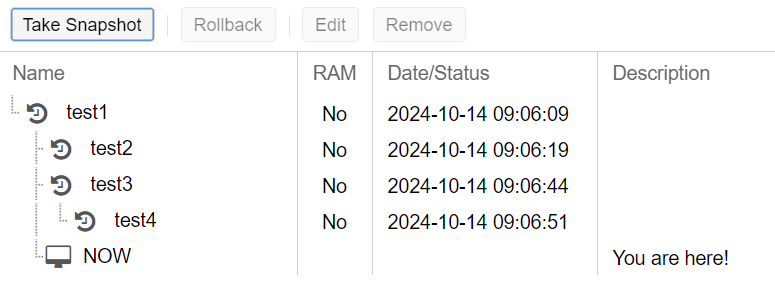
\includegraphics[width=0.8\linewidth]{Proxmox_snapshots.png} % Figure image
	\caption{Snapshot tree in Proxmox} % Figure caption
	\label{fig:Snapshot tree in Proxmox} % Label for referencing with \ref{bear}
\end{figure}

\section{Migration}

\subsection{Migration types}

\paragraph{Cold/Offline Migration} is the process of moving a virtual machine from one physical host to another while the virtual machine is powered off. This is the simplest form of migration and is often used for planned maintenance or to move a virtual machine to a different physical host. Cold migration is the most reliable form of migration as there is no risk of data loss or corruption. However, it does require downtime for the virtual machine, which may not be acceptable for some applications.

\paragraph{Hot/Online/Live Migration} is the process of moving a virtual machine from one physical host to another while the virtual machine is still running. This is a more complex form of migration than cold migration, as it requires the virtual machine to be transferred while it is still in use. Hot migration is often used for load balancing, disaster recovery, or to move a virtual machine to a different physical host without downtime. Hot migration is more complex than cold migration and carries a higher risk of data loss or corruption, but it can be performed without downtime for the virtual machine.

\subsection{Migrating between different hypervisors}

% https://pve.proxmox.com/wiki/Migrate_to_Proxmox_VE
\subsubsection{VMware $\rightarrow$ Proxmox}
Proxmox is able to do manual and automatic import of full VMs from ESXi hosts.

\paragraph{Automatic Import}
Proxmox can automatically import VMs from ESXi hosts. VMs with disks on a VMware vSAN storage cannot be imported automatically, but this can be solved by using a small workaround. Just move the disk to a different storage before importing it to Proxmox.
\begin{figure}[H]
    \centering
    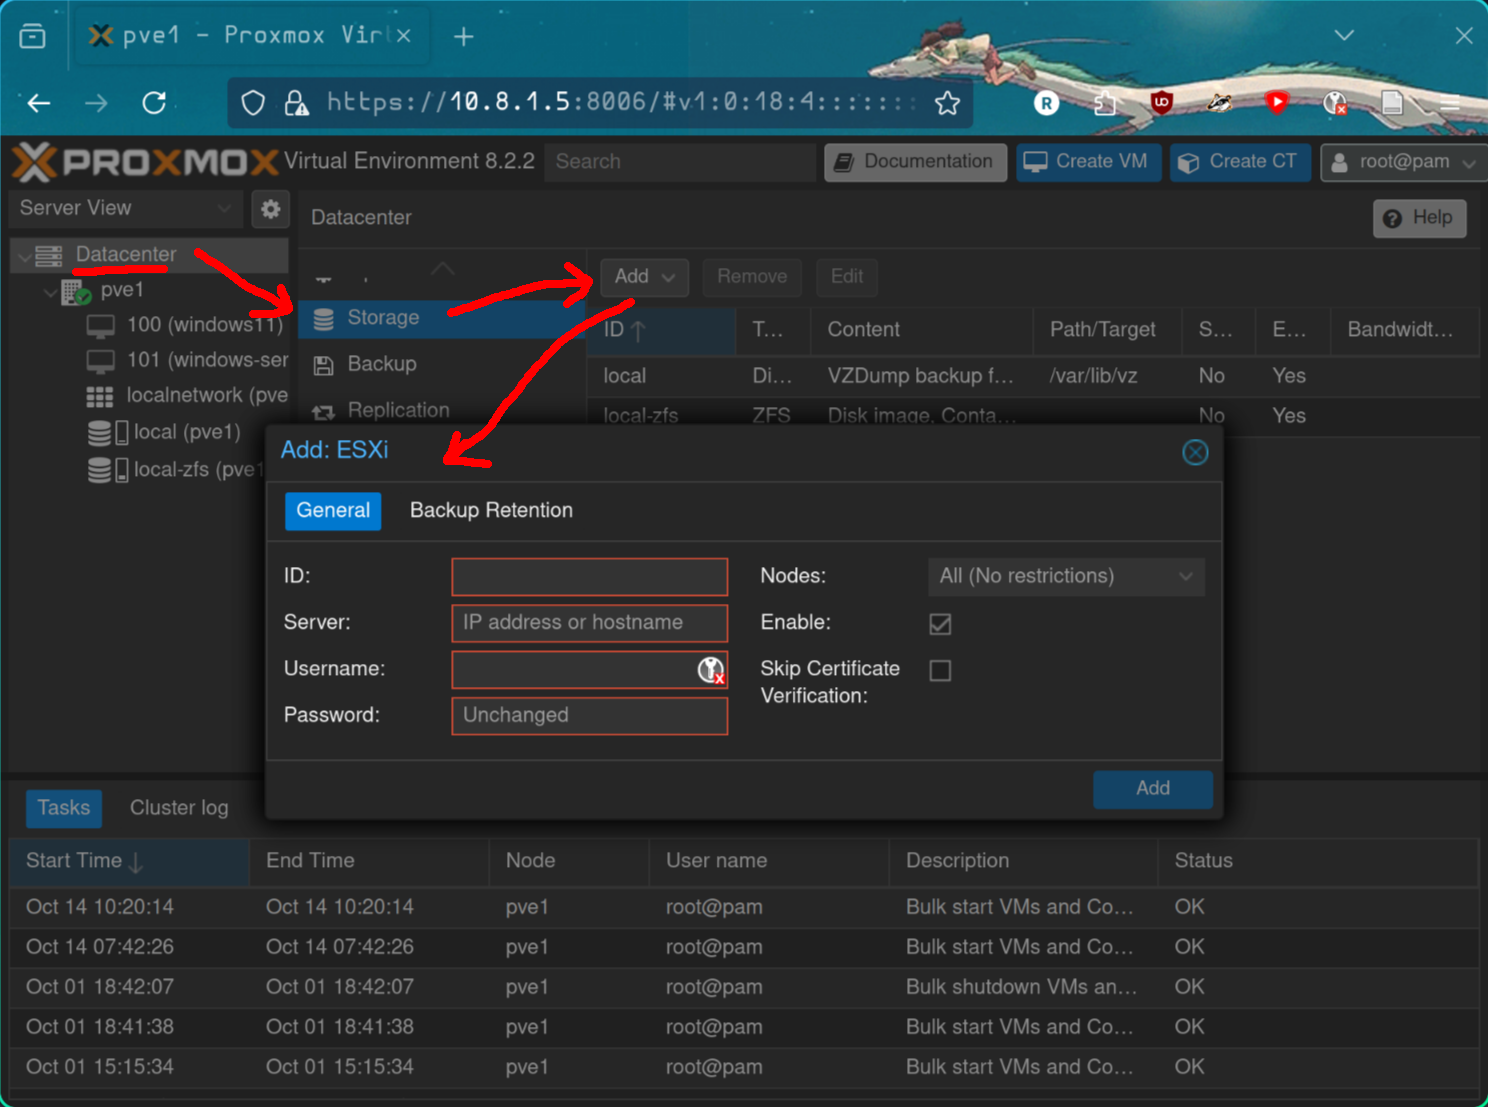
\includegraphics[width=\textwidth]{datacenter_storage_esxi.png}
    \caption{Add ESXi import source to Proxmox}
    \label{fig:proxmox_add_esxi_source}
\end{figure}
To start importing VMs from an ESXi instance it has to be added under Datacenter $\rightarrow$ Storage $\rightarrow$ Add $\rightarrow$ ESXi. \newline
Importing from a vCenter instance is also possible, but will drastically reduce performance.\newline
After adding the ESXi source, the VMs can be imported by selecting the storage in the resource tree and checking the import panel. The VMs can be selected and imported by clicking the import button. You then must select a target storage and network or additionally configure the VM. Now power down the VM on the ESXi host and start the import on Proxmox. The VM will be copied to the Proxmox host and can be started there. You may need to do some post-migration configuration, such as changing the network adapter type or installing VirtIO drivers.

\paragraph{Live Import}
Proxmox also supports live imports. This copies the hard-disk while the VM is still running and syncs all changes asynchronously. When done it automatically starts in Proxmox. While this minimizes downtime it increases the risk of data corruption or loss and is not recommended for production systems.

\paragraph{Mass Imports} should be serialized as much as possible to avoid overloading the ESXi API and potentially interrupting all running imports.
It is generally advised to not import more than 4 VM disks at a time.

\paragraph{Manual Migration}
Manual migration is also possible. The VM must be exported from the ESXi host and then imported to Proxmox. This is more time-consuming and error-prone than automatic migration, but it can be useful for VMs that cannot be migrated automatically.\newline
This can be realized in different ways:
\begin{itemize}
    \item \textbf{Backup} the VM on the ESXi host and restore it on Proxmox.
    \item \textbf{Clone} the VM with a tool like Clonezilla
    \item \textbf{OVF}: Export the VM as an OVF and import it to Proxmox. The \textit{ovftool} can be used to directy import the OVF to Proxmox.
    \item \textbf{Import Disk}: Copy the *.vmdk disk(s) to Proxmox or a shared storage and use the \textit{qm import disk} command to import and convert the disk to the correct target format.
\end{itemize}

\subsubsection{Proxmox $\rightarrow$ VMware}
Migrating VMs from Proxmox to VMware is not as straight forward as the other way around. The VM must be exported from Proxmox and then imported to VMware, as there is no direct import feature in VMware. The following method can be used:
\begin{enumerate}
    \item \textbf{Convert Disk}: The disk must be converted to a format that VMware can read. This can be done with the \textit{qemu-img} tool. 
    e.g. \begin{verbatim}qemu-img convert -f qcow2 -O vmdk disk.qcow2 disk.vmdk\end{verbatim}
    \item \textbf{Create VM}: Next a new VM must be created in VMware which should have the same settings as the VM in Proxmox.
    \item \textbf{Copy Disk}: The converted disk must be copied (e.g. by using scp) to the VMware host and added to the VM. 
    \item \textbf{Boot VM}: The VM can now be started in VMware.
\end{enumerate}

\subsection{Migrating VMs in a cluster}

\subsubsection{Proxmox}
Proxmox supports online/live and offline migration of VMs between nodes in a cluster. 
\paragraph{Preparation} When intending to migrate a virtual machine, it is important to prepare the virtual machine and the target host to ensure a successful migration. The following steps should be taken before migrating a virtual machine:
\begin{itemize}
    \item \textbf{CPU}: Try to choose a CPU-type that is as close to the hardware as possible but supported on all cluster-nodes.
    \item \textbf{Network}: VirtIO NICs are recommended for minimal overhead.
    \item \textbf{Storage}: VirtIO SCSI or VirtIO Block are recommended for minimal overhead. Make sure the target node has enough storage for the VM disk.
    \item \textbf{Memory}: Make sure the target host has enough memory to accommodate the virtual machine.
\end{itemize}

\paragraph{Migrating} to another node can be accomplished by using the CLI or the Web-UI. In the Web-UI it is done by selecting the VM and clicking the migrate button. Disks are either shared or copied early so only the memory and VM state remaing to be synced. The VM will then be moved to another node in the cluster without downtime. Offline migration is also easily possible by shutting down the VM and then migrating it.\newline
Proxmox also supports shared storage, which allows VMs to be migrated between nodes without copying the disk. This is useful for VMs that require high availability or for load balancing. This greatly reduces the time required to migrate a VM, as only the memory and VM state need to be transferred between nodes.

\subsubsection{VMware}
VMware also supports live migration of VMs between hosts in a cluster. This can be accomplished by using vMotion, which allows a VM to be moved between hosts without downtime. vMotion is a complex process that involves transferring the memory and VM state between hosts, as well as updating the network configuration and storage paths. vMotion is a powerful tool that can be used for load balancing, disaster recovery, or planned maintenance. VMware also supports shared storage, which allows VMs to be migrated between hosts without copying the disk.

\section{Datastores}

\section{HA}

\section{Management}


\section{Licensing}

\subsection{Comparison}

\paragraph{Proxmox} 
is \textbf{open-source} and offers all features for free by default for private and/or commercial use. Aditionally, Proxmox offers 4 simple subscription-based models for enterprises which offer technical support and access to the \enquote{Proxmox Enterprise Repository}, which provides reliable updates and security patches. The available subscription models are:
\begin{itemize}
	\item \textbf{Community}:\num{ 110}€/year \& CPU-Socket
	\item \textbf{Basic} \num{340}€/year \& CPU-Socket
	\item \textbf{Standard} \num{510}€/year \& CPU-Socket
	\item \textbf{Premium} \num{1020}€/year \& CPU-Socket
\end{itemize}
All of them offer access to the enterprise repository but they differ in the quality and quantity of their technical support.\newline
An example setup consisting of 3 hosts and a 32-core CPU each will cost from \num{330}€/year to \num{3060}€/year depending on the amount of support wanted. (or nothing on the free edition)


% https://community.veeam.com/blogs-and-podcasts-57/decoding-the-new-broadcom-vmware-vsphere-licensing-packages-for-small-deployments-6398
\paragraph{VMware} requires more complex licensing.\newline
ESXi hosts are licensed with vSphere licenses. There is one main license model and a few older models which are no longer sold but are still supported. The current licensing model is per core licensing with a minimum of 16 cores per CPU. All licenses are sold in different editions:\newline 
\textit{The following prices are based on the MSRP when using a 3-year subscription. VMware offers 1, 3 and 5 year subscriptions with varying prices.}

\subparagraph{vSphere Essentials Plus Kit}
is sold in 96 core license packs and includes vCenter Essentials for up to 3 hosts with a price of \num{35}\$/core/year which totals to \num{3360}\$/year or \num{10080}\$/3-years.

\subparagraph{vSphere Standard} includes vCenter Server Standard and is priced at \num{50}\$/core/year. It does not have a upper limit on hosts or cores. A license with 96 cores would cost \num{14400}\$/3-years 

\subparagraph{vSphere Foundation} includes vSphere Enterprise Plus, vCenter Server Standard, Tanzu Kubernetes Grid, Aria Suite Standard and available Add-On's. Additionally it includes 100GiB of vSAN Enterprise per-core. The price is \num{135}\$/core/year. 
A license with 96 cores would cost \num{38880}\$/3-years.


\subparagraph{Other models,} which are no longer being sold, include: 
\begin{itemize}
	\item per-CPU licensing with a maximum of 32 cores per license. For CPUs with more than 32 cores multiple licenses have to be acquired
	\item pre-VM licensing
	\item vSphere+ capacity based licensing
\end{itemize}

\subparagraph{Evaluation} is possible with a 60-day trial license.
It starts as a free 60-day trial and can be converted to a full license by purchasing a license key. The license key is entered into the vSphere Client and the evaluation license is converted to a full license.

\subsection{Conclusion}

Proxmox's licensing solely provides additional support and updates, while the software itself is free and open-source. 
VMware is proprietary and not free. The licensing is more complex and expensive, but it offers more features and support. 


\clearpage

\tableofcontents

\end{document}
